\documentclass{article}
\usepackage[margin=1in]{geometry}
\usepackage{tikz}
\usepackage{pgfplots}
\pgfplotsset{compat=1.18}
\usetikzlibrary{arrows.meta, positioning, calc, shapes.geometric, decorations.fractals}

\title{LaTeX Image Creation Showcase}
\author{Generated by ChatGPT}
\date{\today}

\begin{document}
\maketitle
\section*{Five Illustrative Images}

% Image 1: Overlapping colourful circles
\begin{figure}[ht]
\centering
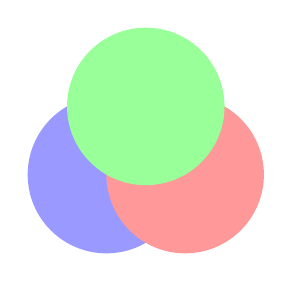
\begin{tikzpicture}
    \fill[blue!40] (0,0) circle (1);
    \fill[red!40] (1,0) circle (1);
    \fill[green!40] (0.5,0.866) circle (1);
\end{tikzpicture}
\caption{Overlapping primary colour circles}
\end{figure}

% Image 2: Sine and cosine waves
\begin{figure}[ht]
\centering
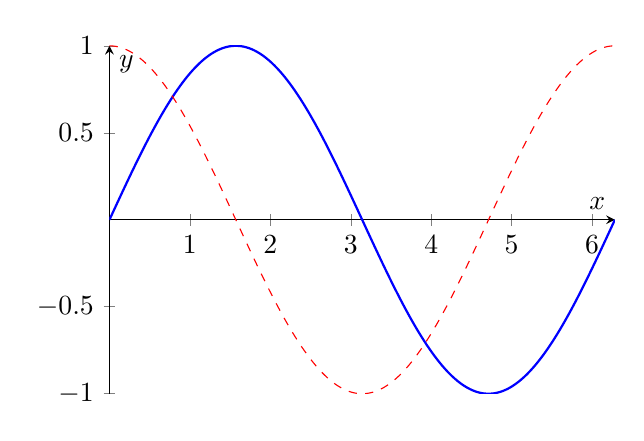
\begin{tikzpicture}
\begin{axis}[width=8cm,height=6cm,axis lines=middle,samples=200,domain=0:6.283,xlabel=$x$,ylabel=$y$]
    \addplot[blue,thick] {sin(deg(x))};
    \addplot[red,dashed] {cos(deg(x))};
\end{axis}
\end{tikzpicture}
\caption{Sine and cosine curves}
\end{figure}

% Image 3: 3D surface plot
\begin{figure}[ht]
\centering
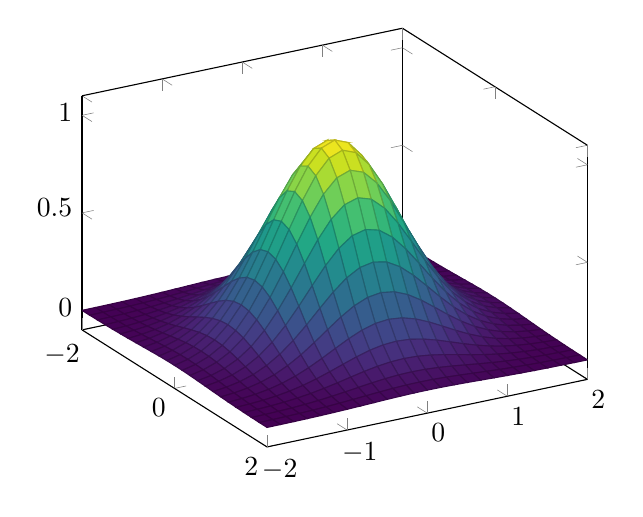
\begin{tikzpicture}
\begin{axis}[view={60}{30},colormap/viridis,width=8cm]
    \addplot3[surf,domain=-2:2,domain y=-2:2,samples=25]{exp(-(x^2+y^2))};
\end{axis}
\end{tikzpicture}
\caption{Gaussian surface}
\end{figure}

% Image 4: Flowchart
\begin{figure}[ht]
\centering
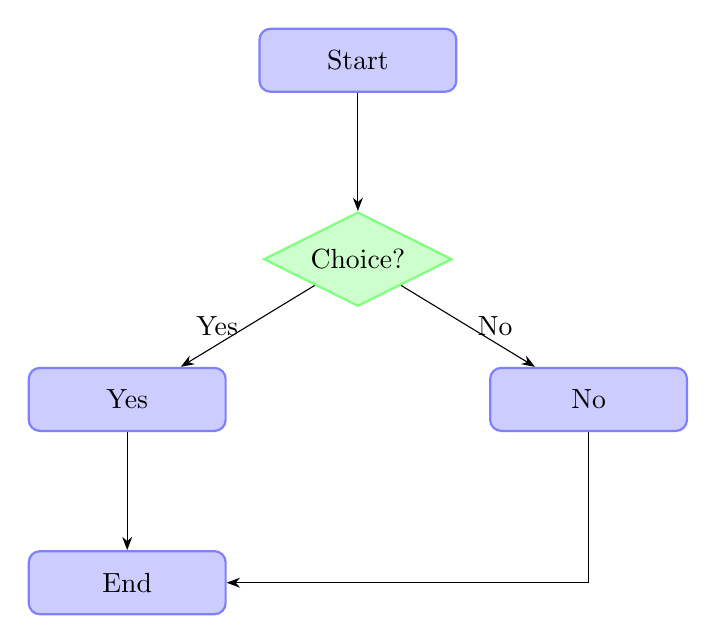
\begin{tikzpicture}[node distance=1.5cm,>=Stealth]
    \tikzstyle{proc}=[rectangle,rounded corners,draw=blue!50,fill=blue!20,thick,minimum width=2.5cm,minimum height=0.8cm]
    \tikzstyle{decision}=[diamond,aspect=2,draw=green!50,fill=green!20,thick,text centered]
    \node[proc] (start) {Start};
    \node[decision,below=of start] (decide) {Choice?};
    \node[proc,below left=of decide] (yes) {Yes};
    \node[proc,below right=of decide] (no) {No};
    \node[proc,below=of yes] (end) {End};
    \draw[->] (start)--(decide);
    \draw[->] (decide)-- node[left]{Yes} (yes);
    \draw[->] (decide)-- node[right]{No} (no);
    \draw[->] (yes)--(end);
    \draw[->] (no)|-(end);
\end{tikzpicture}
\caption{Simple flowchart}
\end{figure}

% Image 5: Koch snowflake
\begin{figure}[ht]
\centering
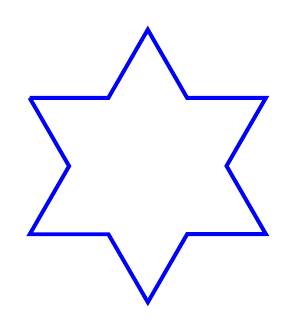
\begin{tikzpicture}[scale=3]
    \draw[blue,line width=0.5mm] decorate [decoration=Koch snowflake] { -- ++(0:1) -- ++(-120:1) -- ++(-240:1) -- cycle};
\end{tikzpicture}
\caption{Koch snowflake fractal}
\end{figure}

\end{document}
